%----------------------------------------------------------------------------------------
\chapter{Validation and Testing} 
\label{chap:validation}
%----------------------------------------------------------------------------------------

This chapter presents the validation and testing of the methods that were before designed and then implemented in this research. 
The accuracy of the results has already been discussed with the error comparison tables in the \cref{chap:design}.
To demonstrate the applicability of this research, instead, the methods are tested on real-life robots, \cref{chap:platforms}.

To achieve these results, some minor adaptations had to be made. For example, the number of input or output dimensions of the network changed to accommodate the joint space of the robots since the monodimensional example given in the design is not enough.

Furthermore, the time scale for the movement primitives has been changed to a longer time period.
The trajectories generated if in cartesian space, were passed to an inverse kinematic algorithm to retrieve the joint space.

Overall, these variations don't impact though what has been discussed and implemented before. 

\newpage
%%%%%%%%%%%%%%%%%%%%%%%%%%%%%%%%%%%%%%%%%%%%%%%%
\section{Partial Skill Combination}
%%%%%%%%%%%%%%%%%%%%%%%%%%%%%%%%%%%%%%%%%%%%%%%%
To test the capabilities of the method developed, the robot selected is the UR10. It is worth noting that the research is not designed specifically for this robot and can be applied to any robot with different specifications. 

The UR10 robot in the setup described in the \cref{chap:platforms} has two main parts: the robot arm that executes the movements and the gripper that grasps the desired object. 

% robot interface
\paragraph{UR10 robot interface} For the sake of completeness, this paragraph briefly describes the Python interface developed to simplify the use of the robot in general and enable this experiment. This interface is available in a \href{https://github.com/igor-lirussi/UR10_robot_interface}{GitHub public repository} \cite{url:UR10repo}. 
The interface acts as a bridge between the user commands and the ROS topics exposed by the robot's computer. 

It implements a series of ROS Subscribers to retrieve the desired data published by the robot and save it into buffer variables. 
Some functions are present to get the variables about the current status of the robot, this makes the read operations fast and not blocking. 

Also, some ROS Publisher nodes are implemented to send commands and information to the robot. These nodes publish data to the robot's defined topics in order to move the device or set the desired settings. Functions are also present here to simplify the calls and send the ROS messages through the nodes implemented. 

% gripper interface
\paragraph{3F Gripper interface} Another codebase repository used in this experiment has been developed to easily interface the gripper to the user and ease its operation. 

This interface is available in a \href{https://github.com/igor-lirussi/Gripper3F_interface}{GitHub public repository} \cite{url:3FGripperrepo}. The code has been developed separately since the gripper is a different entity from the robot and has its own ROS services and IP address. The interface also acts as a connecting link between the Python commands and the ROS services made available by the gripper integrated circuit.

In this case, since the gripper doesn't offer topics but services (see \cref{chap:platforms}) some ServiceProxies are implemented to simplify the operation of this last. The interface offers functions that ease the call of these services to open, close, set the aperture or force of the gripper, get the position, and so on. 

% trajectory recorder and playback
\paragraph{Trajectories recorder and playback} Finally, these two interfaces were used to build a code that allows recording the trajectory in time of the robot's joint positions. Furthermore, the trajectory recorded allows the recording of the cartesian position of the end effector and the gripper aperture.

Moreover, for our experiment, also the code for playing back these trajectories has been written. This work allows the testing in real life of the trajectories generated by the CNMPs architectures developed before. 

\paragraph{Testing}
\begin{figure}
    \centering
    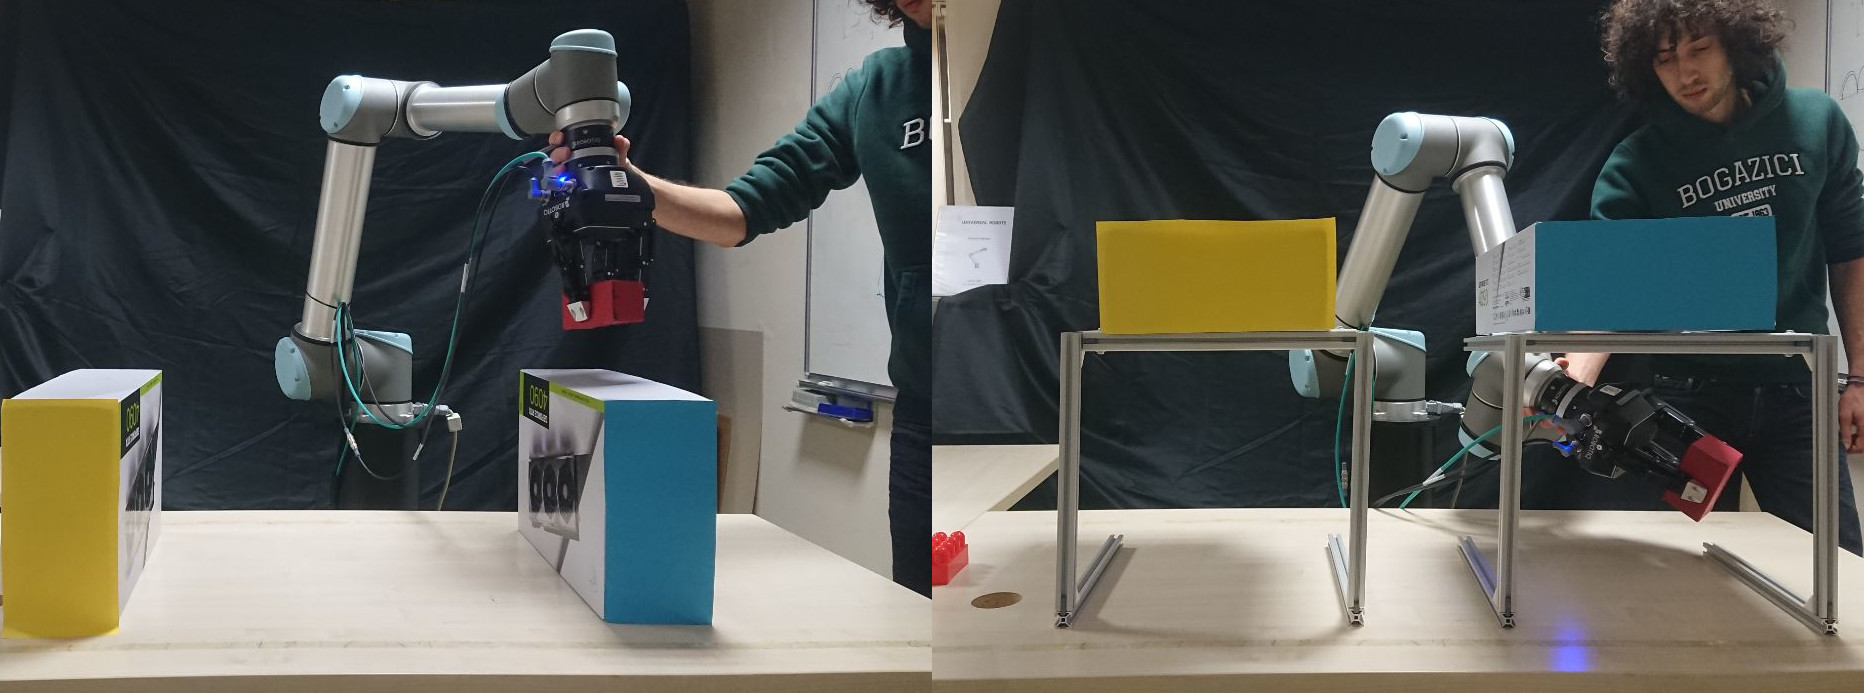
\includegraphics[width=0.9\linewidth]{Images/6Dteach.jpg}
    \caption{ Some moments from learn by demonstration. On the left, action to overcome obstacles. On the right, action to pass under a tunnel. }
    \label{fig:6Dteach}
\end{figure}

The robot was initially used to record some trajectories. This is part of the initial teaching of the "learn by demonstration" process. The trajectories were recorded with the previous code repository developed. 

In \cref{fig:6Dteach}, it is possible to see two moments of this process. On the left image, the capture of an instant from the first action demonstration on how to overcome obstacles. In the right image, another action is taught on how to pass under a tunnel.

\begin{figure}
    \centering
    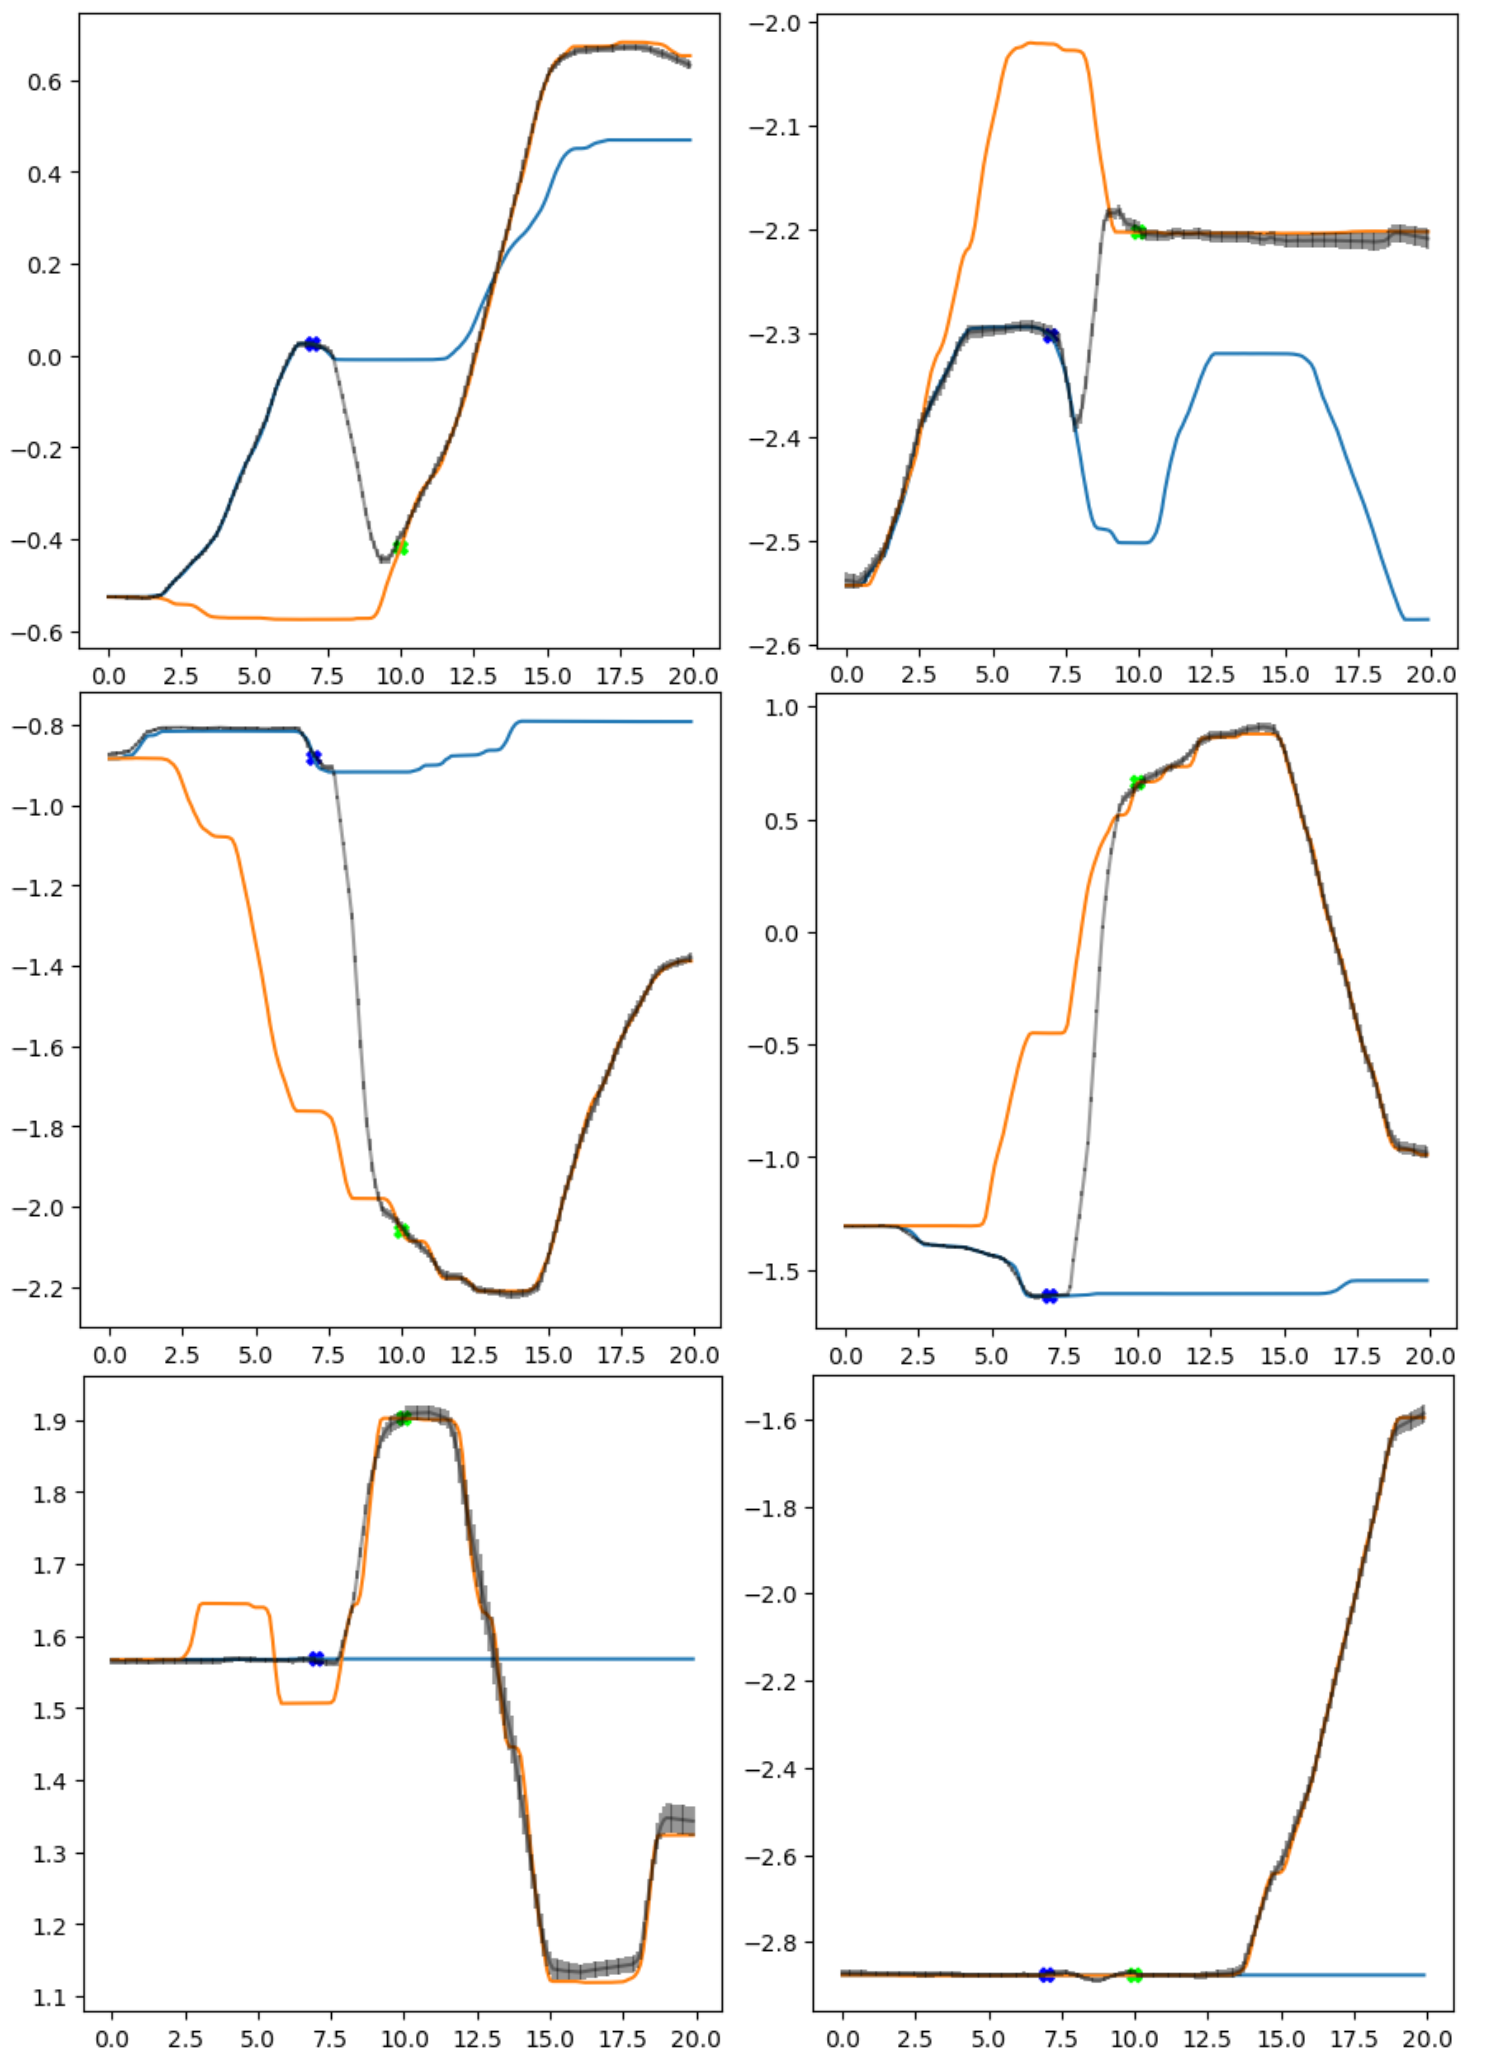
\includegraphics[width=0.9\linewidth]{Images/6Dv.png}
    \caption{ The 6 dimensions of a recorded trajectory on a real robot and the resulting mixed trajectory in grey generated by the network. }
    \label{fig:6Dtrain}
\end{figure}

% extended on 6D 
The UR10 robot has 6 Degrees of Freedom (DoF), so the network input is expanded to 6 dimensions. The choice of joint space is motivated by not dealing later with the inverse kinematics to reproduce trajectories from cartesian space. The six dimensions, one for every joint, of the two trajectories recorded are visible in \cref{fig:6Dtrain}. 

In the figure, the first action of passing over the obstacle is represented by the blue line in the graphs, it indicates the movement of every joint in time. Similarly, the action of passing through a tunnel is visible as the orange line for the same joints in time. 

After training the network with the two trajectories and obtaining a satisfactory result, the method proposed is applied. 
The output trajectory generated is visible in the grey line of every graph. 

It is worth noting that it is not a simple linear transition, but the network captures the non-linearity dependencies across the trajectories and interpolates them accordingly. This results in a mixture of skills that is coherent and maintains the properties of the actions. 

In the graph where the blue joint executes two curves, it is possible to notice this behavior. The trajectory generated does not pass directly from one conditioning point to the other. The final trajectory keeps the properties of the first blue one, descending for a while and then mixing with the orange one. 

\begin{figure}
    \centering
    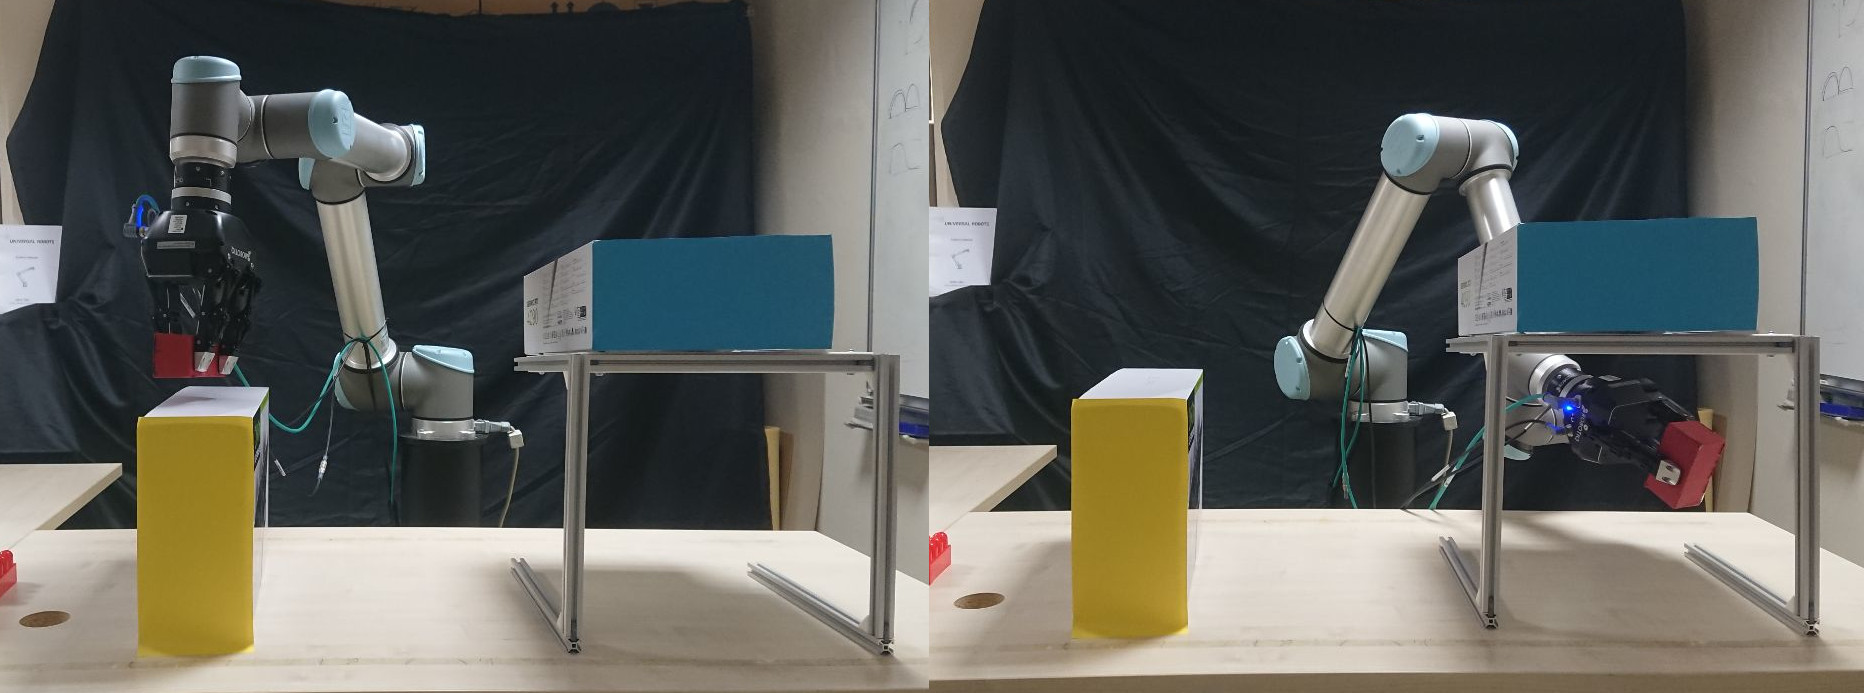
\includegraphics[width=0.9\linewidth]{Images/6Dresult.jpg}
    \caption{ Some instants from the playback of the trajectory generated where the robot successfully completes the combination of the two actions. }
    \label{fig:6Dresult}
\end{figure}

Finally, the trajectory generated is reproduced with the playback code developed. The robot successfully combines the actions and brings the object to the final destination without colliding with the environment. Some moments of the executions are visible in the \cref{fig:6Dresult}. The robot initially overcomes the obstacles with the first part of the action taught, then proceeds to successfully pass through the tunnel, changing its position and orientation.

% pictures trajectories cartesian space training and results?
% pictures of the CNMP failing?

\newpage
%%%%%%%%%%%%%%%%%%%%%%%%%%%%%%%%%%%%%%%%%%%%%%%%
\section{End-To-End Skill Concatenation}
%%%%%%%%%%%%%%%%%%%%%%%%%%%%%%%%%%%%%%%%%%%%%%%%
For the End-To-End Skill Concatenation, the robot used for real-life testing is Baxter Robot, \cref{chap:platforms}.
It is crucial to highlight that the research is not exclusive to this specific robot though. The platform has been used only to demonstrate the real applicability and efficacy of the work presented. 

Moreover, part of the choice to use this platform instead of UR10 is indeed to prove that the models and methods developed are platform-independent and can be implemented on any robot. 

Baxter robot has a complete set of interaction and Learning from Demonstration capacities. Moreover, the manipulation capabilities, although limited by the two-finger parallel grippers, are easier to integrate with the expert demonstrations and trajectory recordings. The robot has two buttons on the hands that are easy to press and link with the gripper position. The end effectors are light and simple to move. 

This part of the research implies the concatenation of primitives, so many different demonstrations. Furthermore, the skills are related to the environment and manipulation of objects, so it's crucial to have a platform that is easy to interact with. For this reason, the Baxter robot has been selected for this research demonstration.

% Baxter interface
\paragraph{Baxter robot interface} Another repository implemented along with the previous ones for the experiments in real life is the interface for the Baxter robot in Python 3. This work was driven by the need for Python 3 compatible functions since Baxter has an interface, but it is only Python 2, and it's not compatible with the majority of ML frameworks nowadays. This interface is available in a \href{https://github.com/igor-lirussi/baxter-python3}{GitHub public repository} \cite{url:Baxterrepo}. 

Baxter exposes a ROS system as well, with ROS topics and services. For this reason, the interface uses nodes and ServiceProxies to send messages or call actions in the robot. To speed up the reading process, there are buffer variables for the data that the robot publishes. This has been especially useful in the recording stage since it increased the resolution of the recordings from 10Hz to 100Hz.

The robot exposes plenty of options, being designed for collaborative tasks. It has the possibility to set the joint position, to set the cartesian position of the end effector, and to retrieve these last ones. Moreover, it's possible to set and get the gripper position or the display image, or read the data from the infrared sensors and cameras in the hands. 

All these options are available in the Python 3 interface developed. Moreover, some examples are present of how to move the robot or control from the keyboard, how to get the data from the sensors and cameras, and how to use the inverse kinematic services and the grippers. 

% trajectory recorder and playback
\paragraph{Trajectories recorder and playback} Lastly, in the interface developed previously, it is possible to find also the code to record the trajectories of the arms of the robot and play them back. 

The recorder waits for the pressing of a button and starts to save current time and the position of the joints at the frequency desired. Moreover, the recorder also saves the end effector cartesian position and orientation for later comparison. 

The gripper position and force read are also saved in the data for every timestep. This is useful for manipulation tasks that require handling objects. 

Furthermore, a trajectory visualizer for cartesian and joint space has been developed as well. The code enables the user to see the movement primitive in 3D and check the correctness of the data recorded or about to be played. The 3D visualization of the trajectory can be optionally surrounded by five graphs for each individual dimension of the cartesian or joint space. The color of the points in 3D corresponds to the gripper aperture. 

Lastly, the complementary code for the playback of trajectories enables the robot to move precisely from the data provided. The trajectories can be previously recorded or generated with a network. For this reason, this code was especially useful in testing this research. 

% Baxter picking objects and object detection
\paragraph{Baxter detecting and reaching objects} 
Another code repository was developed to complement the research done with a method that can bring the robot actuator to the initial position. In the discussion presented, the robot arm has to be in an initial state, from which possible and meaningful actions are generated. Here we briefly propose a method that can reach the initial state. This will make the demonstration more complete from the side of a spectator and independent from an expert who has to guide the robot in the initial state.

The code and the neural network model weights are available in a \href{https://github.com/igor-lirussi/Baxter-Robot-ObjDet}{GitHub public repository} \cite{url:BaxterrepoObjDet}.

The method developed consists of putting the robot arm in a pose from which the cameras in the hands are leveraged to acquire the RGB image of the table below. Subsequently, the objects present will be detected with the use of a neural network for object detection, namely YOLO. The robot will use the given positions of the objects to move the arm slightly toward the one desired. The inverse kinematics service of the robot takes care of computing the pose for the new cartesian position. The process repeats till the infrared (IR) sensor of the hand detects the distance of the object as "graspable". At this point, the gripper closes and the object is reached for further desired manipulation.

This code has been used in the research as a viable way to get to the initial pose and the object. Many other more complicated approaches are possible. Reached the initial state, then demonstrated the method presented are demonstrated.   



\paragraph{Testing}